\chapter{Nonlinear Optics}

%Descrição de polarização não-linear, potencial atómico. Descrição no bulk de geração de terceiro harmônico. 
\section{Optical Polarization}
An important subject of optics science to describe the interaction between light and matter is the dipole moment per unit volume, which is called polarization. In a dielectric medium the polarization occurs mainly due induced dipoles.

\begin{figure}[h!]
    \centering
    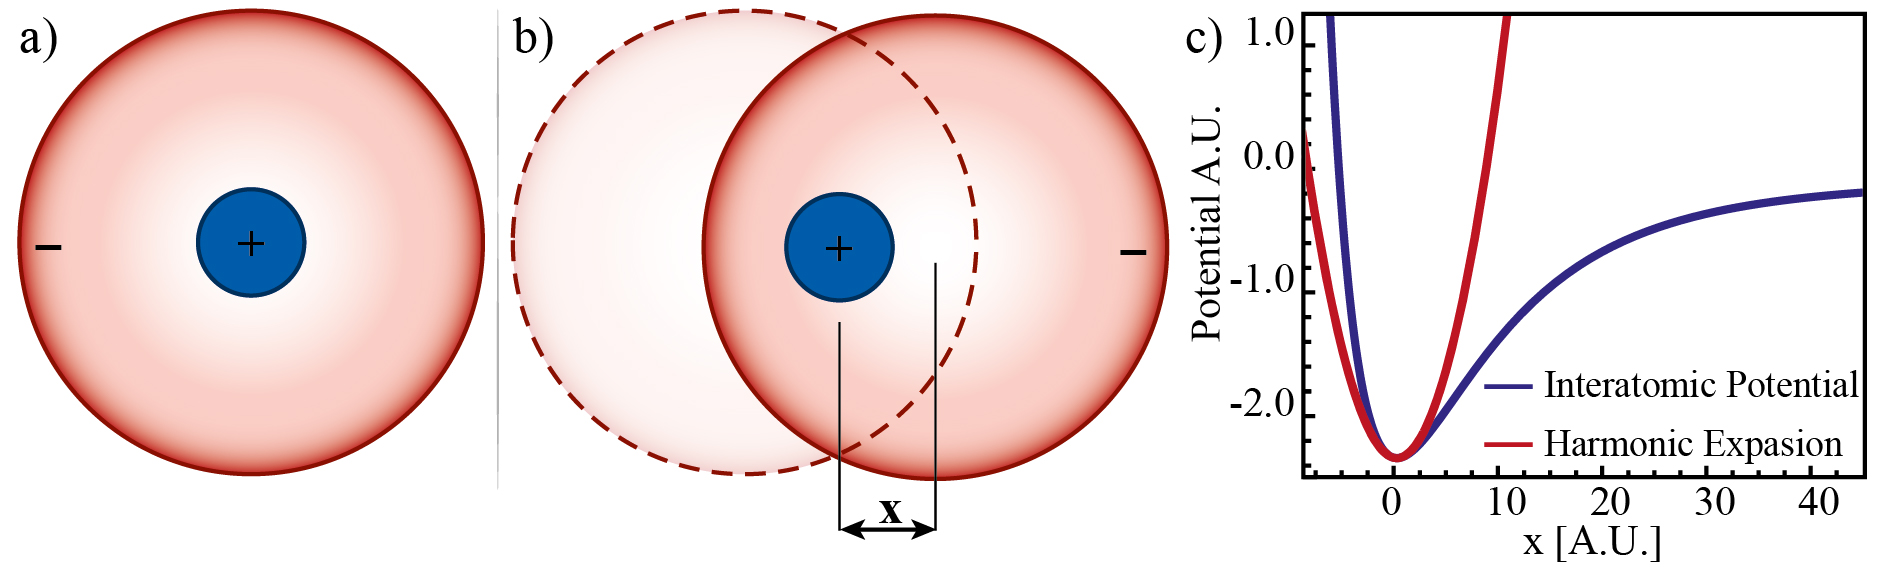
\includegraphics[width = 16cm]{figuras/Dissertation_atomic_polarization.jpg}
    \caption{\textbf{a) Atom in equilibrium:} the spherical symmetry of the atom makes it neutral for any external electric field. \textbf{b) Atom out of equilibrium:} If a strong enough external electric field are applied, it cause a displacement $x$ which generate a dipole with moment proportional on $x$. \textbf{c) Interatomic potential:} For a small displacement $x$ it is possible to approach the potential as an parable.}
    \label{fig:polarization}
\end{figure}
Lets consider a neutral atom placed in an electric field $\vec{E}$. A priori the electric field shouldn't affect the atom, which is true only due the spherical configuration of the atom, Fig~\ref{fig:polarization}a
. However, the electric field allow a displacement in the equilibrium position of the electron, creating a ionized dipole, as shown in Fig~\ref{fig:polarization}b. It is easy to show that the dipole moment is proportional to displacement distance with the form
\begin{equation}
    \vec{p} = q\vec{d}.
\end{equation}
Wheres $q$ is the charge of the nucleus. 

When a weak external electric field is considered (if compared with the atomic electric field), we can approach the atomic potential to a parabolic, as show in Fig~\ref{fig:polarization}c. The restoring force, therefore, is linear with distance. In such model, the polarization $\vec{p}$ is linear with the external electric field
\begin{equation}
    \vec{p} = \alpha \vec{E}.
\end{equation}
Where $\alpha$ is a constant called atomic polarization and depends on the atomic structure. This simple model is, in fact, in well agreement with experimental result.  

The result for a single atom can easily extend for a solid body applying the principle of  superposition, this way
\begin{equation}
    \vec{P} = \epsilon_0\chi^{(1)}\vec{E}.
\end{equation}
Where $\susce{1}$ is the linear suceptibility and depends on the atomic configuration.

The assumption of weak external electric field implies in a small displacement, otherwise we can't assume a parabolic potential due to the anharmonic form of the interatomic potential. 

In order to formulate a more general model, lets consider the motion of a electron in an anharmonic potential. Let $x$ be the displacement of the electron from the equilibrium position, we have
\begin{equation}
    \ddot{x} + 2\gamma\dot{x} + \omega_0^2x+ax^2+bx^3 = -eE(t)/m.
    \label{eq:motion_equation_electron}
\end{equation}
Here we assumed a applied electric field is given by $E(t)$, the electron charge as $-e$, a damping force of the form $-2m\gamma\dot{x}$ and a restoring force given by
\begin{equation}
    F_\text{restoring} = -m\omega_0^2x -max^2 -mbx^3, 
\end{equation}
where $a$ and $b$ are parameters that characterizes the strength of the nonlinearity. This restoring force corresponds to a potential energy with the form 
\begin{equation}
    U(x) = -\int F_\text{restoring} dx = \frac{1}{2}m\omega_0^2x^2 +\frac{1}{3}max^3 +\frac{1}{4}mbx^4.
\end{equation}

\begin{figure}[h!]
    \centering
    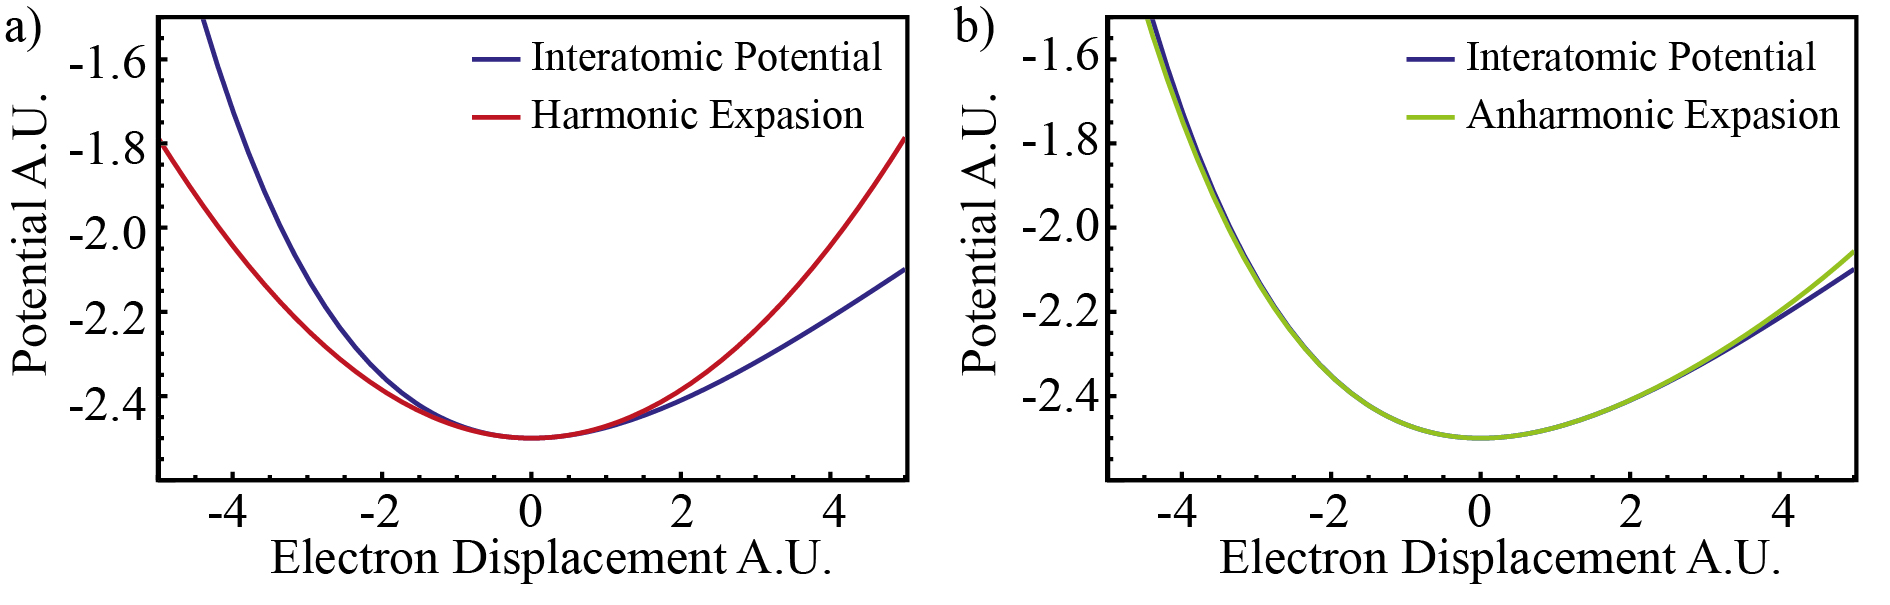
\includegraphics[width = 16cm]{figuras/Dissertation_interatomic_expassion.jpg}
    \caption{\textbf{a) Harmonic expansion:} The assumption of a parabolic potential are only valid if the Electron displacement are small when compared with the atom radius.\textbf{b) Anharmonic expansion:} Consider high order therms, anharmonic therms, for the expansion of the potential lead to a well agreement even when considered higher displacement.}
    \label{fig:expanssion}
\end{figure}
We can solve Eq.\ref{eq:motion_equation_electron} applying perturbation theory. Lets replace $E(t)$ by $\lambda E(t)$,
\begin{equation}
    \ddot{x} + 2\gamma\dot{x} + \omega_0^2x+ax^2+bx^3 = -\lambda eE(t)/m,
    \label{eq:pertubed_equation_electron}
\end{equation}
where $\lambda$ is continuous and ranges between zero and one. We seek for solutions in the form of power series of $\lambda$, that is 
\begin{equation}
    x = \lambda x^{(1)} + \lambda^2 x^{(2)} + \lambda^3 x^{(3)} +....
    \label{eq:x_pertubation_expanssion}
\end{equation}
This procedure give us a set of equations.
\begin{subequations}
    \begin{align}
        \ddot{x}^{(1)} + 2\gamma\dot{x}^{(1)} + \omega_0^2x^{(1)} &= -eE(t)/m,\label{eq:first_order_pertubation}\\
        \ddot{x}^{(2)} + 2\gamma\dot{x}^{(2)} + \omega_0^2x^{(2)}+a\left(x^{(1)}\right)^2 &= 0,\label{eq:second_order_pertubation}\\
        \ddot{x}^{(3)} + 2\gamma\dot{x}^{(3)} + \omega_0^2x^{(3)}+     2ax^{(1)}x^{(2)} +b\left(x^{(1)}\right)^3 &= 0\label{eq:thirdt_order_pertubation}...    
    \end{align}
\end{subequations}

It is easy to see that the first order equation, Eq \ref{eq:first_order_pertubation}, give us the same result as the unperturbed system. If considered a harmonic electric field with module $E(t) = Ee^{-i\omega t}$, for the steady-state we have
\begin{equation}
    x^{(1)}(t) = \tilde{x}^{(1)}e^{-i\omega t}.
\end{equation}
The amplitude have the form
\begin{equation}
    \tilde{x}^{(1)} = -\frac{e}{m}\frac{E}{\omega_0^2-\omega^2-2i\omega\gamma}.
\end{equation}

Now we are able to rewrite the Eq \ref{eq:second_order_pertubation} as a driver harmonic oscillator with drive force give by 
\begin{equation}
    ma\left(x^{(1)}\right)^2 = ma\left(\tilde{x}^{(1)}\right)^2e^{-i2\omega t}.
\end{equation}
Here is where things start to get interesting. Our system was initially drove by a harmonic force with frequency $\omega$, the anharmonic form of the interatomic potential bring forth a drive force with frequency $2\omega$, which can be notice in the expression
\begin{equation}
    \ddot{x}^{(2)} + 2\gamma\dot{x}^{(2)} + \omega_0^2x^{(2)} = a\left(\tilde{x}^{(1)}\right)^2e^{-i2\omega t}.
\end{equation}
The steady-state solution have the form
\begin{equation}
    x^{(2)}(t) = \tilde{x}^{(2)}e^{-i2\omega t}.
\end{equation}
Applying the Fourier transform it is easy to find that
\begin{equation}
    \tilde{x}^{(2)} = -\frac{a\left(\tilde{x}^{(1)}\right)^2}{\omega_0^2 - (2\omega)^2-2i\gamma2\omega}.
\end{equation}

The same procedure for Eq \ref{eq:thirdt_order_pertubation} give us a perturbation with frequency $3\omega$, with the form 
\begin{equation}
    x^{(3)}(t) = \tilde{x}^{(3)}e^{-i3\omega t},
\end{equation}
where
\begin{equation}
    \tilde{x}^{(3)} = -\frac{b\left(\tilde{x}^{(1)}\right)^3 + 2 a \tilde{x}^{(1)}\tilde{x}^{(2)}}{\omega_0^2 - (3\omega)^2-2i\gamma3\omega}.
\end{equation}

The Eq \ref{eq:x_pertubation_expanssion} now give us a important inside. Even know that the drive force due the external electric field are well defined with frequency $\omega$, the solution for the motion of the electron around the rest position give us a harmonic series
\begin{equation}
    x(t) = \lambda \tilde{x}^{(1)}e^{-i\omega t} + \lambda^2 \tilde{x}^{(2)}e^{-i2\omega t} + \lambda^3 \tilde{x}^{(3)}e^{-i3\omega t} +....
\end{equation}
Here I define the component drive by the external force as the fundamental mode of the motion of the electron and the high order terms are called second and third harmonic (later, we will apply this nomenclature for the optical mode).  

This calculus can easily be extended to a vector analyse, along with the definition of dipole moment we can write
\begin{equation}
    \vec{p} = q\left(\lambda\vec{\tilde{x}}^{(1)}e^{-i\omega t}+\lambda^2\vec{\tilde{x}}^{(2)}e^{-i\omega t}+\lambda^3\vec{\tilde{x}}^{(3)}e^{-i\omega t}+... \right).
\end{equation}
For a solid body we have
\begin{equation}
    \vec{P} = \epsilon_0\chi^{(1)}\vec{E} + \epsilon_0\chi^{(2)}\vec{E}^2+\epsilon_0\chi^{(3)}\vec{E}^3+....
\label{eq:nonlim_pol}
\end{equation}
Note that the nonlinear susceptibility, $\chi^{(2)}$, $\chi^{(3)}$, are tensors.

The main reason behind the math showed in this section is to make clear and intuitive that the generation of high orders harmonics occurs only due the interaction between an incident wave and the matter. This will be an important statement further below. 

Now that I have convinced you that an anharmonic potential are able to generate high orders harmonic in the motion of the electrons leading to nonlinear terms for the polarization.% we can check what the effect upon a propagating electromagnetic wave.

\section{Wave Equation}

Let consider the effect of polarization upon the wave equation for a nonlinear optical medium. Starting with Maxwell's equations

\begin{subequations}
    \begin{alignat}{2}
        &\nabla\cdot\vec{D}  &&= 0,\\
        &\nabla\cdot\vec{B}  &&= 0,\\
        %\nabla\times\vec{E} &=  i \omega\vec{B}\\
        &\nabla\times\vec{E} &&= -\frac{\partial\vec{B}}{\partial t},\\ 
        %\nabla\times\vec{H} &= -i \omega\vec{D}\nabla\times\vec{E}
        &\nabla\times\vec{H} &&= \frac{\partial\vec{D}}{\partial t}.
    \end{alignat}
    \label{eq:max_eq}
\end{subequations}

We consider a nonmagnectic material, hence
\begin{equation}
    \vec{B} = \mu_0 \vec{H}
\end{equation}

%Otherwise, by consider a nonlinear medium, for the electric field we have
%\begin{equation}
%    \vec{D} = \epsilon_0\vec{E} + \vec{P}
%\end{equation}
%where $\vec{P}$ are given by Eq \ref{eq:nonlim_pol}.
%
Applying some math, is possible to rewrite the Maxwell's equations in wave equation form for the electric field 
\begin{equation}
    \nabla^2\vec{E} - \frac{1}{\epsilon_0 c^2}\frac{\partial^2}{\partial t^2}\vec{D} = 0
\end{equation}
As we considered a nonlinear optical medium, we shall use
\begin{subequations}
    \begin{align}
        \vec{D} &= \epsilon_0\vec{E} +\vec{P},\\
        \vec{P} &= \vec{P}^{(1)} + \vec{P}^{(NL)}.
    \end{align}
\end{subequations}
In order to simplify the math, we split the polarization vector $\vec{P}$ in a linear part, given by $\vec{P}^{(1)} = \epsilon_0\chi^{(1)}\vec{E}$, and a nonlinear part $\vec{P}^{(NL)}$ given by the nonlinear terms of the Eq~\ref{eq:nonlim_pol}, so we have

\begin{equation}
    \nabla^2\vec{E} +\frac{\n^2}{c^2}\frac{\partial^2}{\partial t^2}\vec{E} = -\frac{1}{\epsilon_0 c^2} \frac{\partial^2}{\partial t^2}\vec{P}^{NL}.
    \label{eq:wave_equation_nonlinear}
\end{equation}
The refraction index, n, can be write as $\n^2= 1 + \chi^{(1)}$ and is a function of the frequency.

The fallowing procedure can be applied for how many nonlinear terms you wish, but, since this is not the focus of this dissertation, I will proceed considering only the second order term. In such case

\begin{equation}
    \vec{P}^{NL} = \vec{P}^{(2)} = \epsilon_0\bar{\bar{\chi}}^{(2)}\vec{E}\vec{E}.
    \label{eq:nonlinear_polarization}
\end{equation}
Where the total electric field are the sum of different frequency waves, for the second harmonic generation we have
\begin{equation}
    \vec{E} = \vec{E}_1 + \vec{E}_2.
    \label{eq:total_field}
\end{equation}
Here, just for formality, I explicitly write the tensorial and vectorial form of the nonlinear polarization and fields, however we will consider the case of a $z$ propagating wave in a isotropic medium, which enable us to suppress the vectorial and tensorial notation, dealing just with scalar equations.

Lets consider the case of a incident plane wave with frequency $\omega_1$, we can write the components of the total electric field as    
\begin{equation}
    E_i = A_ie^{i(k_i-i\omega_i t)} + c.c., \text{ for $i = 1,2$}
\end{equation}
where $\omega_2 = 2\omega_1$ and $k_i = \omega_i/\n_ic$. 

We are assuming that there is no other process beside second harmonic generation, resulting in a nonlinear polarization with two components, so that   
\begin{equation}
    P^{(2)} = P_1e^{-i\omega_1 t}+P_2e^{-i\omega_2 t}
    \label{eq:nonlinear_polarization_harmonic_form}
\end{equation}

Due to the harmonic time dependence of the field, we can use $\frac{\partial}{\partial t} = -i\omega$, then the Eq~\ref{eq:wave_equation_nonlinear} can be write for each frequency, 
\begin{equation}
    \frac{\partial^2}{\partial z^2}E_i +\frac{\omega_i^2}{c^2}\n_i^2 E_i = -\frac{\omega^2}{\epsilon_0 c^2} P_i
\end{equation}
Calculating the scalar form of the Eq~\ref{eq:nonlinear_polarization} and Eq~\ref{eq:total_field}, comparing with Eq~\ref{eq:nonlinear_polarization_harmonic_form} it is possible, and quit easy, to find that
\begin{subequations}
    \begin{align}
        P_1 &= 2\chi^{(2)} A^*_1 A_2e^{i(k_2-k_1)z}\\
        P_2 &= \chi^{(2)} A_1^2e^{i2k_1z}
    \end{align}
\end{subequations}

The full wave equation for each component are give, therefore, by 
%\begin{subequations}
%    \begin{align}
%       \frac{\partial^2}{\partial z^2}A_1e^{ik_1z} +\frac{\omega_1^2}{c^2}\n_1^2 A_1e^{ik_1z} &= -2\frac{\omega_1^2 \chi^{(2)}}{\epsilon_0 c^2} A^*_1 A_2e^{-i\Delta kz}\\
%       \frac{\partial^2}{\partial z^2}A_2e^{ik_2z} +\frac{\omega_2^2}{c^2}\n_2^2 A_2e^{ik_2z} &= -\frac{\omega_2^2\chi^{(2)}}{\epsilon_0 c^2} A_1^2e^{i\Delta k z}
%    \end{align}
%\end{subequations}
\begin{subequations}
    \begin{align}
       \frac{\partial^2}{\partial z^2}A_1 +\frac{\omega_1^2}{c^2}\n_1^2 A_1 &= -2\frac{\omega_1^2 \chi^{(2)}}{\epsilon_0 c^2} A^*_1 A_2e^{-i\Delta kz}\\
       \frac{\partial^2}{\partial z^2}A_2 +\frac{\omega_2^2}{c^2}\n_2^2 A_2 &= -\frac{\omega_2^2\chi^{(2)}}{\epsilon_0 c^2} A_1^2e^{i\Delta k z}
    \end{align}
    \label{eq:coupled_wave_equation_SHC}
\end{subequations}
Here I defined 
\begin{equation}
    \Delta k = 2k_1 - k_2.
\end{equation}

Solution for coupled-wave equation have already been demonstrated, however I not interested in a analytic form for the amplitude hence the system Eq~\ref{eq:coupled_wave_equation_SHC} was solved using numerical methods.

\begin{figure}[h!]
    \centering
    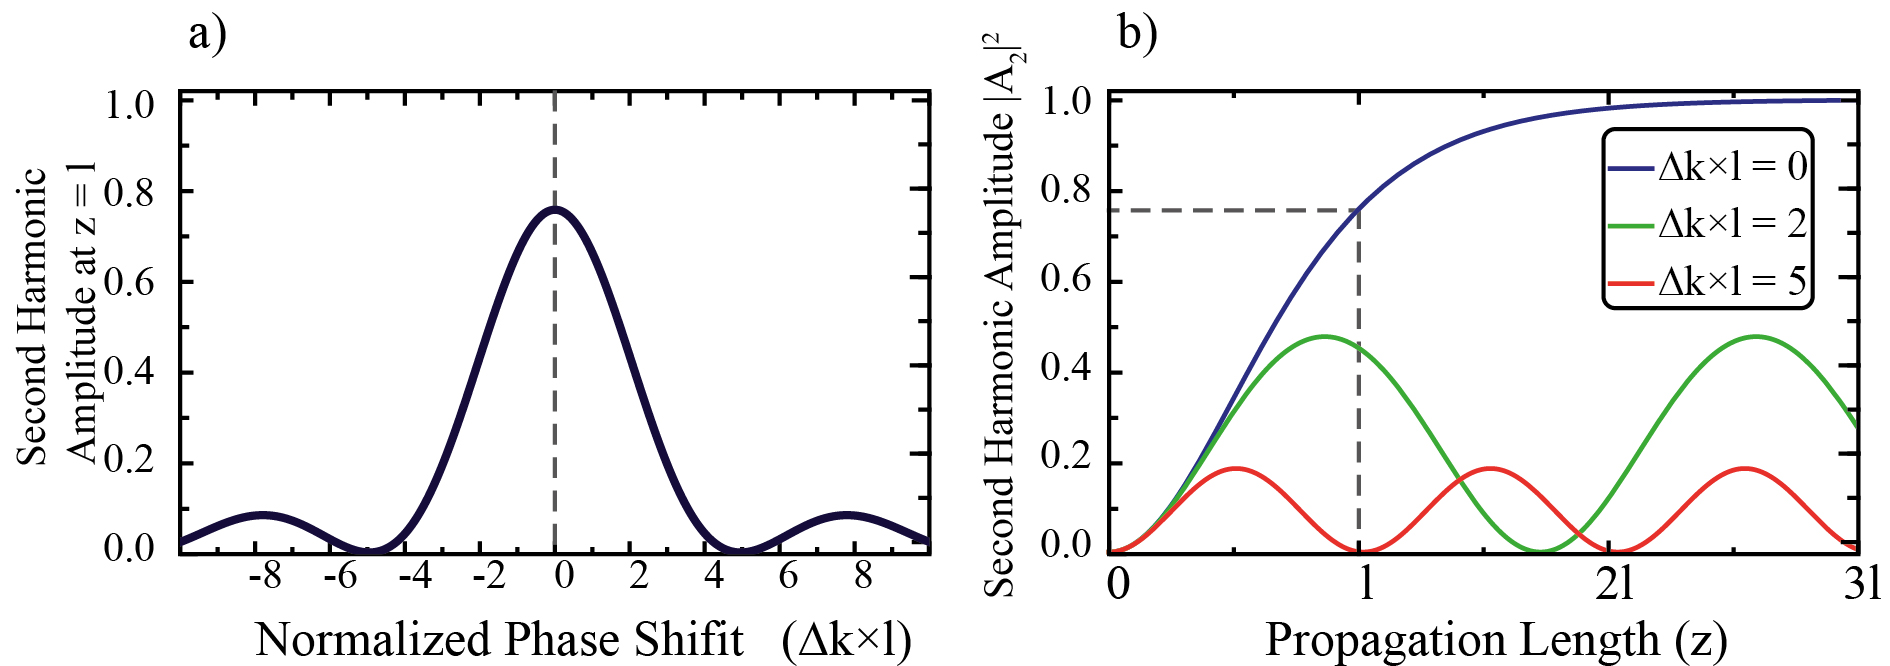
\includegraphics[width = 16cm]{figuras/Dissertation_coppled_eq_sol.jpg}
    \caption{\textbf{Coupled-wave equation numerical solution: a)} Modulus of the second harmonic amplitude, $|A_2|$, in function of $\Delta k \times l$ for $z = l$. \textbf{b)} Modulus of the second harmonic amplitude, $|A_2|$, in function of $z = l$ for different values of $\Delta k \times l$.}
    \label{fig:model_solution}
\end{figure}

In order to normalize the equations I define $l$ as the distance where, for $\Delta k = 0$, the amount of $75\%$ of the energy in the fundamental mode have been transferred for the second harmonic mode. 

Analysing the results presented in Fig~\ref{fig:model_solution} it is possible observe two interesting, and indeed important, behaviors. The graphic Fig~\ref{fig:model_solution}a) shows that the amount of energy in the second harmonic model is maximum for $\Delta k = 0$, moreover, the Fig~\ref{fig:model_solution}b) shows that the stand steady are only reached for $\Delta k = 0$, any other value of $\Delta k$ lead to an oscillation in function of the propagation distance.

Now is a good moment for introduce a new definition. Lets suppose we have two different optical modes, $A_j$ and $A_l$, wheres $j,l \in \mathbb{N} $ and $j<l$, with frequency $\omega_j$ and $\omega_l$ and constant of propagation $k_j$ and $k_l$, if
\begin{subequations}  
    \begin{alignat}{3}
        &\Delta\omega &&= l \omega_j - j \omega_l & &= 0,\\
        &\Delta k &&= l k_j - j k_l & &= 0,
    \label{eq:phase_matc}
    \end{alignat}
\end{subequations}  
we then call this modes in a phase matching.

\section{Conclusion}
We spent this chapter to do some superficial math, it is possible find in literature much more details about the theory of nonlinear polarization and high order harmonic generation. 

However we got two, although obvious, important conclusion. First, was seen that the harmonic generation are result of the interaction between just the light and matter. Second, two modes are in phase matching only if both $\Delta \omega$ and $\Delta k$ are simultaneous zero.

This two conclusions will be better applied when we look for third harmonic generation in  modes confined in cavities. But, before, lets describe the theory of optical cavities.  